\documentclass[12pt]{article}
\usepackage{listings}
\usepackage[colorlinks=true,pagebackref,linkcolor=blue]{hyperref}
\usepackage{graphicx}
\usepackage{tikz}
\textwidth=7in
\textheight=9.5in
\topmargin=-1in
\headheight=0in
\headsep=.5in
\hoffset  -.85in

\lstset{
basicstyle=\footnotesize\ttfamily,
language=bash,
upquote=true,
breakatwhitespace=true,
columns=fullflexible,
keepspaces,
%numbers=none,
tabsize=3,
frame=blrt,
framextopmargin=5pt,
showstringspaces=false,
extendedchars=true
}

\pagestyle{empty}

\renewcommand{\thefootnote}{\fnsymbol{footnote}}

\begin{document}



\begin{center}
{\bf AMS 550.400 \quad HW SET 1\quad  Due Date:  Oct 8}\\
\vskip.2in
{\footnotesize Last Compiled on \today}
\end{center}

\setlength{\unitlength}{1in}

\begin{picture}(6,.1) 
\put(0,0) {\line(1,0){6.25}}         
\end{picture}

 

\renewcommand{\arraystretch}{2}


\vskip.25in
\noindent\textbf{Problem 1 (10 pts):}  
Assume that you are starting from ``scratch'' at the directory \verb+~/+.
Provide a sequence of git/bash commands that yields a git folder with 
a commit history such that:
\begin{itemize}
\item the \emph{master} branch has commits $A$, $B$, $C$, $X$ and $D$,
\item the \emph{alt} branch has commits $A$, $B$, $X$,
\end{itemize}
Suppose that you are currently working on \texttt{master} branch. Draw 
its commit history graph (i.e., the graph portion of the output of
\verb+git log --graph --oneline+).  Next, assume that 
you are on \texttt{alt} branch. Draw its commit history graph.  


\noindent\textbf{}
\\
In this problem, I used the following code:  
  \\  cd \textasciitilde/550400
  \\  mkdir \textasciitilde/550400/honda
  \\  cd \textasciitilde/550400/honda
  \\  git init
  \\  vi main.txt
  \\  git add .
  \\  git commit -m "A is done"
  \\  vi main.txt
  \\  git add .
  \\  git commit -m"B is done"
  \\  git checkout -b alt
  \\  vi main.txt
  \\  git add .
  \\  git commit -m"X is done"
  \\  git checkout master
  \\  vi main.txt
  \\  git add .
  \\  git commit -m "C is done"
  \\  git merge alt
  \\  vi main.txt
  \\  vi main.txt
  \\  git add .
  \\  git commit -m "D is done"
  \\  git log --graph --oneline
  \\  git checkout alt
  \\  git log --graph --oneline
  \\  git push https://github.com/zhendanzhu/honda.git master
  \\  git push https://github.com/zhendanzhu/honda.git alt

\begin{figure}[h]
    \begin{center}
        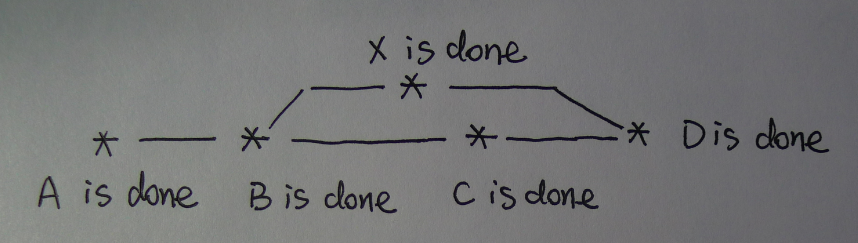
\includegraphics{grapha.png}
    \end{center}
    \caption{The history graph for master branch}
    \label{fig:branch}
\end{figure}

\begin{figure}[h]
    \begin{center}
        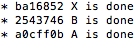
\includegraphics{graphb.png}
    \end{center}
    \caption{The history graph for alt branch}
    \label{fig:branch}
\end{figure}


\vskip.25in
\noindent\textbf{Problem 2 (10 pts):}
Assume that you are starting from ``scratch'' at the directory \verb+~/+.
Provide a sequence of git/bash commands that yields a git folder and 
\begin{itemize}
\item configure your git with your name and your email address,
\item set up an alias for each of the git remotes listed below:
\begin{verbatim}
git://github.com/nhlee/550400.stanza1.git 
git://github.com/nhlee/550400.stanza2.git 
git://github.com/nhlee/550400.stanza3.git 
\end{verbatim}
Assume that each remote contains exactly single commit with 
a txt file for a single (different) stanza,
\item pull to combine three stanzas of a poem,
\item after the first pull, add the title of the poem,
\item after the second and third pull, resolve the merge conflict,
\item after resolving the third pull merge conflict, push the result
  to your (newly created) remote repository. 
\end{itemize}

\noindent\textbf
mkdir newpoem
\\cd  \textasciitilde/newpoem
\\git config --global user.name "zhendanzhu"
\\git config --global user.email zhendanzhu@hotmail.com
\\git remote add stanza1 git://github.com/nhlee/550400.stanza1.git 
\\git remote add stanza2 git://github.com/nhlee/550400.stanza2.git 
\\git remote add stanza3 git://github.com/nhlee/550400.stanza3.git 
\\git init
\\git checkout master
\\git pull stanza1 master
\\vi  main.txt
\\git add .
\\git commit -m " add a title "
\\git checkout -b alt1
\\git pull stanza2
\\git checkout master
\\git merge alt1
\\vi main.txt
\\git add .
\\git commit -m "resolve conflict1"
\\git checkout -b alt2
\\git pull stanza3
\\git checkout master
\\vi main.txt
\\git add .
\\git commit -m "resolve conflict2"
\\git remote add origin https://github.com/zhendanzhu/poemmerge.git
\\git push -u origin master

\newpage
\noindent\textbf{Problem 3 (40 pts):}
Consider a team of four students, say, $A$, $B$, $C$ and $D$, 
who just started working 
on writing a \texttt{latex/beamer} file, say \texttt{main.tex}, 
for a class presentation of their work statement.  
Assume that they do not wish to coordinate their schedules for a
concurrent group meeting (both virtually and physically).  
Assume that:
\begin{itemize}
\item $A$ is in charge of \emph{Introduction},
\item $B$ is of \emph{Problem Statement}, 
\item $C$ is of  \emph{Timeline},
\item $D$ is of \emph{Deliverable} part of the presentation.  
\end{itemize}
In other words, their contributions to \texttt{main.tex} do not overlap.
Then, 
\begin{itemize}
\item first, devise a work flow strategy for the team so that they can
  collaborate asynchronously using \texttt{git},
\item next, devise yet another \texttt{git} strategy different from your earlier
  proposal.  
\end{itemize}
Finally,
\begin{itemize}
\item discuss the strength and weakness of each of your proposed strategies in terms of merge
conflicts resolution,
\item make the final recommendation.  
\end{itemize}
In order to answer this question, \emph{build}
a mathematical model, \emph{following} the guideline from IMM. 
Use Section 1.4 and Section 1.5 of IMM as \emph{role models}.    
For example, you are to identify which variables  are exogenous 
and which are endogenous.  More specifically, among other things, 
in your model, is the preamble part of \texttt{main.tex} an endogenous 
or exogenous variable?  
Note also that in addition to this issue, there are other issues that
you are to consider.  So, \emph{be sure to consult IMM}. 


\vskip.25in
\noindent\textbf{Problem:}
 Resolve the conflicts between different editions based on workflow design.
\\ When will be the conflicts? Well, if C is behind the others, say haven't finish the timeline while A B D have already start the work. Or they have done the work on different editions, when they merge them together, they will find conflicts in the contents done by other people. The best way to solve it is by keep each teammate informed of the confict so that they can solve it in time. However, given that each person may have flexible schedule, I think the better way is to reduce the total number of merging and marked on the part to be merged.\\
\noindent\textbf{ Outline for the model:}
\\Proposal plan 1: We will have only one branch, i.e, all the work will be done in master branch, and each time one finished his work, he can push it back to the master's branch. 

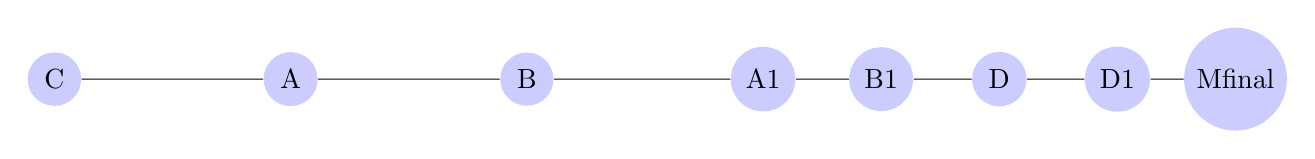
\begin{tikzpicture}
  [scale=1.5,auto=left,every node/.style={circle,fill=blue!20}]
  
  \node (n1) at (0,2)  {C};
  \node (n2) at (2,2)  {A};
  \node (n3) at (4,2)  {B};
  \node (n4) at (6,2)  {A1};
  \node (n5) at (7,2)  {B1};
  \node (n6) at (8,2)  {D};
  \node (n7) at (9,2)  {D1};
  \node (n8) at (10,2)  {Mfinal};
  \foreach \from/\to in {n1/n2,n2/n3,n3/n4,n4/n5,n5/n6,n6/n7,n7/n8}
    \draw (\from) -- (\to);
\end{tikzpicture}\\

Stength:keep each person's newest edition updated in time.
\\ Weakness: the workflow will be a mess if each one of the team submit the unfinished part. It needs many merges during the process, which will lower the efficiency of the project.
\\Proposal plan 2: Since $A $B $C $D have relatively independent part of the project, each one can work on his/her own branch first, and merge to the master's branch when it is done. Considering different person may work asynchronously. Each time there's a conflict in merging, we can simply keep what it is for our own part and wait for the other one to update their part . Since C is responsible for timeline, it can be done independently in one file. If eventually C finished first, then A B D can follow the timeline to do their part and update their work in a fixed schedule. If C haven't finish his part, then A B D can work in a free way as long as they pull the latest edition from the github before they start working on their part. 
\\Strength: Each one of the team will have its independent part, so that we can reduce the times of merge. Keep completeness of each one's work while make a clear outline for the whole process. 
\\Weakness, the number of conflicts will be a headache when B merged his file with master branch if  A, C, D  updated their part during B's work. So one person may need to solve the conflicts of merge of several person's editions. 

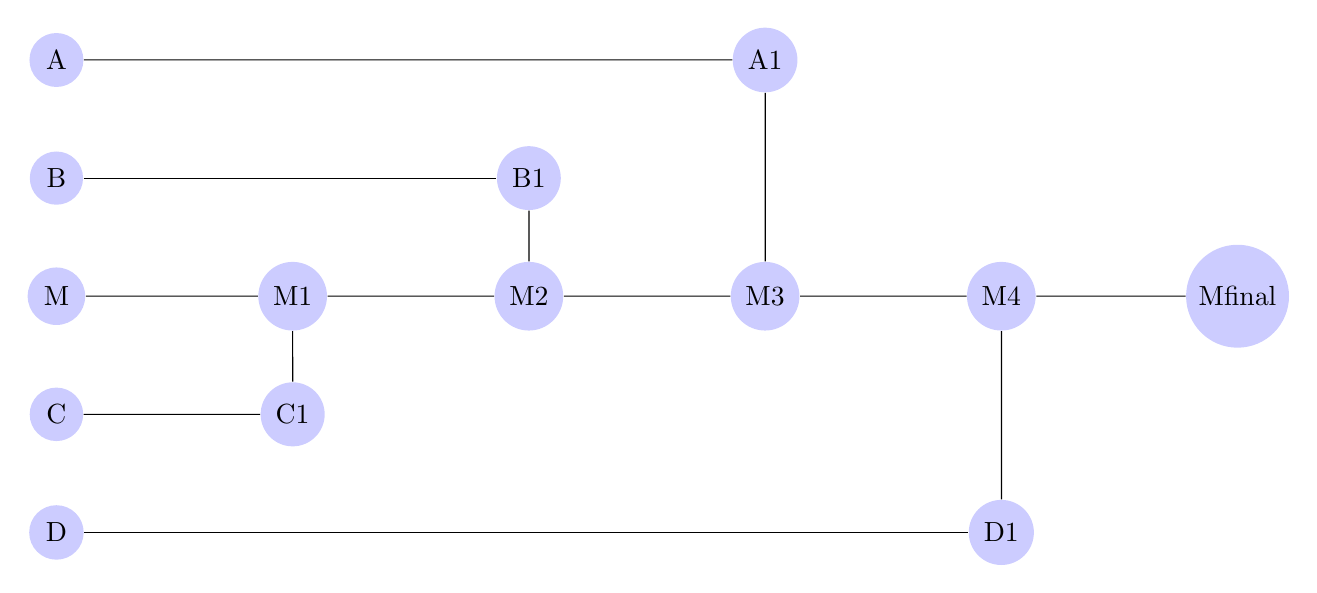
\begin{tikzpicture}
  [scale=1.5,auto=left,every node/.style={circle,fill=blue!20}]
  \node (n1) at (0,4) {A};
  \node (n2) at (0,3)  {B};
  \node (n3) at (0,2)  {M};
  \node (n4) at (0,1) {C};
  \node (n5) at (0,0)  {D};
  \node (n6) at (2,2)  {M1};
  \node (n7) at (4,2)  {M2};
  \node (n8) at (6,2)  {M3};
  \node (n9) at (8,2)  {M4};
  \node (n10) at (10,2)  {Mfinal};
  \node (n11) at (6,4) {A1};
  \node (n12) at (4,3) {B1};
  \node (n13) at (2,1) {C1};
  \node (n14) at (8,0) {D1};


  \foreach \from/\to in {n3/n6,n6/n7,n7/n8,n8/n9,n9/n10,n1/n11,n2/n12,n4/n13,n5/n14,n11/n8,n12/n7,n13/n6,n14/n9}
    \draw (\from) -- (\to);

\end{tikzpicture}

Final Recommendation: Plan 2 will be good, because it has an individual branch for each person. Each one of team can keep track of others work ( individual branch) while have a clean clue about the process of the whole project( master branch).



\vskip0.25in
\noindent\textbf{Problem 4 (aka.\ Fair Play, 40 pts):}
Answer the following question:
\begin{verse}
Is the tennis game fair?
\end{verse}
Note that unlike Problem 3, this question is vaguely stated.
This is intensional, whence to begin, you will first need to clarify
what exactly your question is.
You may use the class discussion on this particular 
problem, but you \emph{may not} directly refer to our 
discussion.  Instead, formulate the model carefully but concisely in 
your own words.   

\vskip0.25in

\noindent\textbf{Problem:}  
\\ Is the game fair?A general standard for this is if the roles of the competitors are reversed, their probability of
winning does not change. Our original problem can be breaked down to several parts: whether the player who is first to serve will be in advantage?  What will be the chances for the first game server to win the match given the probability of winning rate for each ball? And to what extent will the advantage be?

\noindent\textbf{Outline for the model:}   We are going to calculate the probability that the first server to win the match. According to tennis rule, one player delivers the ball to start the game, called server; and one who receives the ball is called receiver. We simplified the rule by stating that each tennis game into a rule that any person who wins two straight points will win the game.And there are 6 games in a match. The possible condition for a game is as following:

\begin{figure}[h]
    \begin{center}
        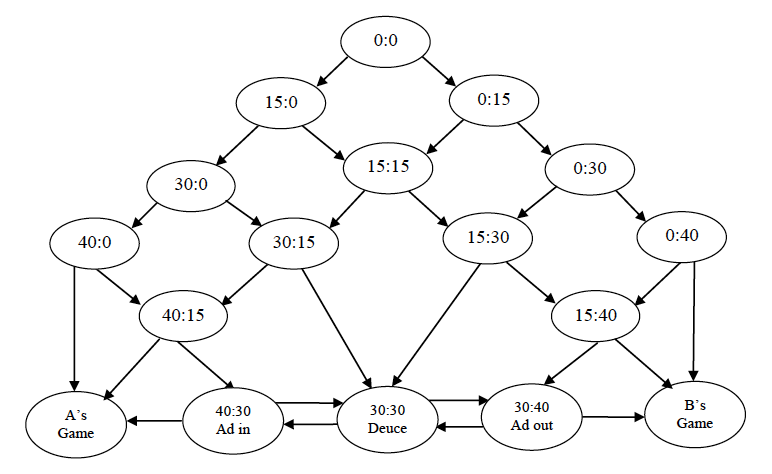
\includegraphics[scale=0.6]{graph2.png}
    \end{center}
    \caption{The graph for possible score results}
    \label{fig:branch}
\end{figure}


 Condition: For both players, the chances for the server to win is P, and the probability for the receiver is 1-P. 

Analysis: Whether the game is fair or not depends on the server's winning rate P on each ball. For each player, the chance to win a game is the same, it equals $Q=P^2/(P^2+(1-P)^2)$. The chance to lose the game is $(1-P)^2/(P^2+(1-P)^2)$.  If P>1/2, then the winning rate for the server in each game is bigger than 1/2. Given the rule for winning a tennis match is the one who wins the fisrt 6 games will win. The final score can be "6:0", " 6:1" , "6:2" ...The total chance for the first server to win is 


\[
 \sum_{k=0}^{5} {k+5\choose 6}{Q^6(1-Q)^k}
\]

The value for this function is show as following 

\begin{figure}[h]
    \begin{center}
        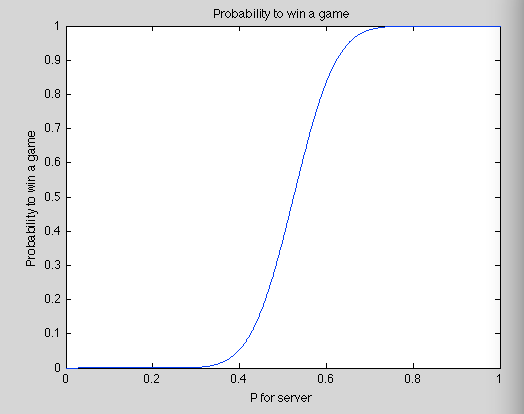
\includegraphics[scale=0.8]{graph3.png}
    \end{center}
    \caption{The graph for possible winning rate}
    \label{fig:branch}
\end{figure}

Code is as following(Figure 4):
\begin{figure}[h]
    \begin{center}
        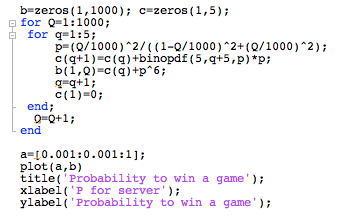
\includegraphics{code.png}
    \end{center}
    \caption{Matlab code}
    \label{fig:branch}
\end{figure}

\noindent\textbf{}
We will conclude that the fairness of tennis depends on the capability of each play.The stronger the server, the more advantage he will have in the tennis game. Especially, when P=1/2, the chance for each player to win equals 1/2. The game is absolutely fair. On the other hand, if the receiver is strong enough that the chance for him to win each point exceeds 1/2, then he will have the advantage. So tennis is a fair game if each person has a relatively equal winning rate in both server's game and receiver's game.


\vskip0.25in
\noindent\textbf{Final Remarks about Problem 3 \& Problem 4:} 
They are open-ended problems.  However, your scores will be determined
by how well do you follow the exposition style outlined by IMM and
WMA.  For both problems, your write-up should be 
\begin{itemize}
\item self-contained,
\item covering all four parts of Section 1.3 of IMM,
\item paying a particular attention to any causal relation that you
  might be investigating, following Chapter 3 of WMA,
\item answering questions that are explicitly asked in the problem statements.
\end{itemize}
For Problem 3, focus mostly on Step 2 and Step 3 of Section
1.3 of IMM.  For Problem 4, focus mostly on Step 1 and Step
2.  For each problem, minimum 1 pages and maximum 2 pages.
\end{document}
